%---------------------------------------------------------
%This block of code is for the table of contents after
%the title page
%---------------------------------------------------------

\section[Intro]{Introduction}

%---------------------------------------------------------
%Changing visibwility of the text

\begin{frame}
    \frametitle{Title of your slide}
    \begin{itemize}
        \item \small{Example of text in an item bullets.}
    \end{itemize}
    \vfill
    %\centering

    \footnotetext[1]{\fullcite{Louis2016}} %To add your reference, copy your library (.bib file) to the presentation folder.
\end{frame}

%---------------------------------------------------------


%---------------------------------------------------------
%Example of the \pause command
\begin{frame}
    \frametitle{Example of pause command}
    In this slide \pause
    
    the text will be partially visible \pause
    
    And finally everything will be there
\end{frame}
%---------------------------------------------------------

\section[Methods]{Methods}

%---------------------------------------------------------
%Highlighting text
\begin{frame}
    \frametitle{Methods}
    \begin{itemize}
        \item Data acquisition
    \end{itemize}
    \begin{table}
    %\caption{CNS pathologies involving BBB dysfunction.}
    %\label{tab:tabela_1}
        \resizebox{\textheight}{!}{% Resize table to fit within \linewidth horizontally
        \begin{tabular}{|P{0.3\textwidth}|P{0.3\textwidth}|P{0.3\textwidth}|P{0.3\textwidth}|}%{\linewidth}{l|X}
            \hline % Linha superior
            Text & Text & Text & Text mm\textsuperscript{2} \\ \hline % Linha do meio 
            Text & Text & Text & Text \\ \hline
            Text & Text & Text & Text \\ \hline
            Text & Text & Text & Text \\ \hline
            \multicolumn{4}{|c|}{Example of multi columns merged!!!} \\ \hline
            %\\\bottomrule % Linha inferior
        \end{tabular}}
    \end{table}
        %Adapted from \cite{Abbott2010}
        \vfill
        \begin{columns}
        \column{0.6\textwidth}
        \begin{itemize}
            \item Example of adding two columns format to the slide
            \begin{itemize}
                \item Major item 1: 
                \begin{itemize}
                    \item sub-item1;
                    \item sub-item2;
                    \item sub-item3;
                    \item sub-item4;
                    \item sub-item5.
                \end{itemize}  
            \end{itemize}
        \end{itemize}

        \column{0.4\textwidth}
        \begin{itemize}
            \item Text for collumn 2; 
            \parnote[\(\dagger\)]{\label{note:dagger}Example of footnote} for MATLAB.
            \item Another item.
        \end{itemize}
        
        
    \end{columns}
    \parnotes

\end{frame}
%---------------------------------------------------------

\section[Cap1]{Results \& Discussion}

%---------------------------------------------------------
%Two columns
\begin{frame}
\frametitle{Title for results slide}

%\begin{figure}[!htb]
    %\centering
    %\includegraphics[width=\linewidth,height=0.85\textheight,keepaspectratio]{Figures/figure.png}
    %\label{justalabel}
%\end{figure}
\end{frame}

\begin{frame}
    \frametitle{Discussion}
    \begin{itemize}
        \item item1;
        \item item2;
        \item item3;
        \item item4;
        \item item5.
    \end{itemize}
\end{frame}



\begin{frame}
    \frametitle{Example of adding multiple figures to the slide}
    \begin{figure}
        \begin{minipage}{0.65\textwidth}
            \centering
            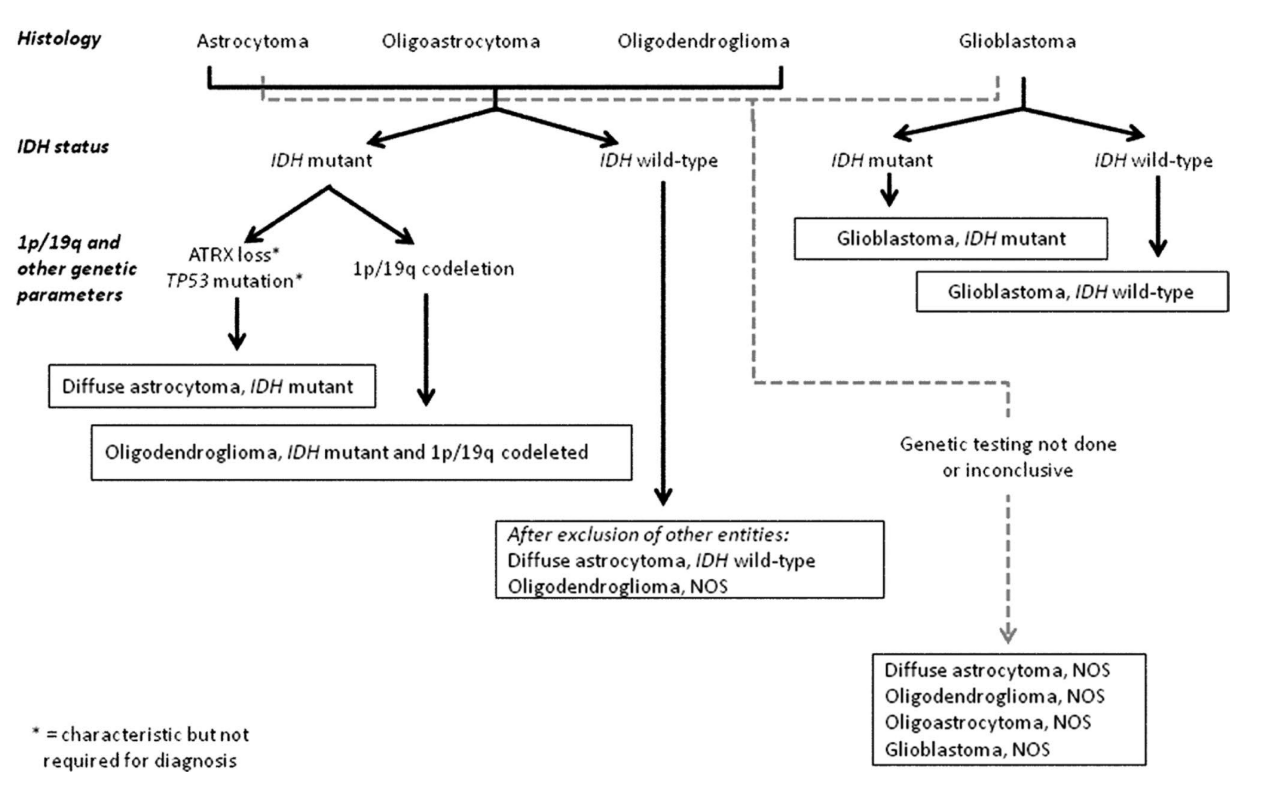
\includegraphics[width=\linewidth,height=0.4\textheight,keepaspectratio]{Figures/gliomaHist.png}
            %\caption{Exemplo de figura embutida no texto}
            \label{fig1}
        \end{minipage}\hfill
         \begin{minipage}{0.35\textwidth}
            \centering
            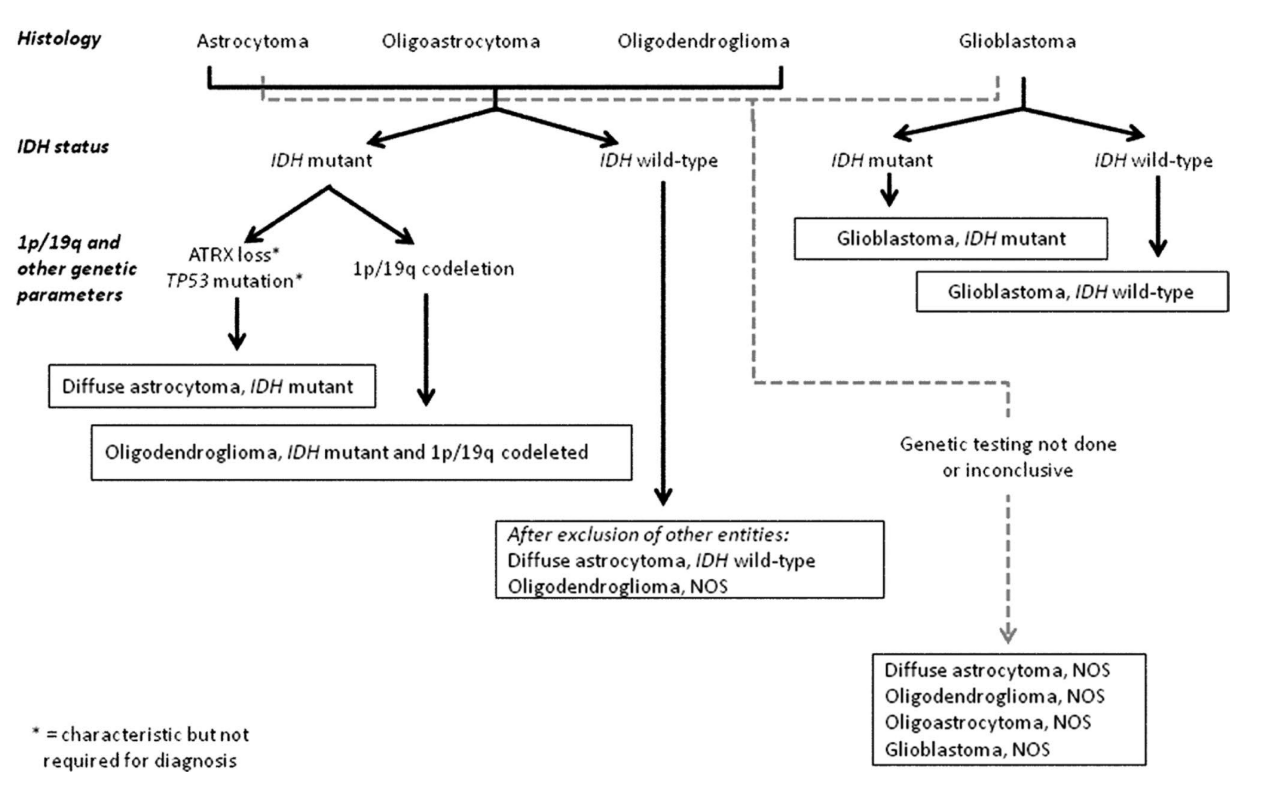
\includegraphics[width=\linewidth,height=0.4\textheight,keepaspectratio]{Figures/gliomaHist.png}
            %\caption{Exemplo de figura embutida no texto}
            \label{fig2}
        \end{minipage}
    \end{figure}
\end{frame}

%---------------------------------------------------------

\section[Conclusions]{Conclusions}

%---------------------------------------------------------

\begin{frame}
    \frametitle{Conclusions}
    \begin{block}{\centering \textbf{Take Home Message 1}}
        \centering \small{Key message 1.}
    \end{block}
    
    \begin{block}{\centering \textbf{Take Home Message 2}}
        \centering 
        \begin{itemize}
            \item \small{Item 1} 
            \item \small{Item 2}
        \end{itemize}
    \end{block}
     
\end{frame}

\begin{frame}
    \frametitle{Aknowledgements}
    \begin{figure}
        \begin{minipage}{0.6\textwidth}
            \centering
            \huge{\textbf{Thank you!}}
        \end{minipage}\hfill
        \begin{minipage}{0.4\textwidth}
            \centering
            \begin{minipage}{0.35\textheight}
                
\includegraphics[width=\linewidth,height=1\textheight,keepaspectratio]{Figures/fapesp.png}                
            \end{minipage}
            \begin{minipage}{0.35\textheight}
                
\includegraphics[width=\linewidth,height=1\textheight,keepaspectratio]{Figures/cnpq.png}
            \end{minipage}
            \begin{minipage}{0.35\textheight}
                
\includegraphics[width=\linewidth,height=1\textheight,keepaspectratio]{InradFrametitle.png}
            \end{minipage}
        \end{minipage}
    \end{figure}
\end{frame}